\section{Introduction}
%\begin{wrapfigure}{r}{0.5\textwidth} % Ajuste la largeur selon le besoin
 %   \vspace{-0.5cm} % Ajustement vertical
  %  \centering
   % \resizebox{0.5\textwidth}{!}{ % Réduire la taille
    %    \begin{tikzpicture}[scale=1, every node/.style={scale=0.9, anchor=east}]

	
    %}
   % \caption{\underline{Construction de $\mathcal{SA}_{T}$}}
   % \vspace{-0.5cm} % Ajuster l'espace sous la figure
%\end{wrapfigure}

\subsection{Environnement du stage}

Ce travail est la synthèse de mon stage de première année de Master, durant lequel j'ai intégré l'équipe de la professeure Thérèse Commes du laboratoire Bio2M,
 rattaché à l’Institut national de la santé et de la recherche médicale (INSERM). J'ai eu la chance d'être accompagné dans mon apprentissage par Anthony Boureux, enseignant-chercheur.
L'équipe est en collaboration étroite avec des services cliniques et des plateformes hospitalières, ce qui favorise évidemment l’innovation et la résolution de questions liées au champ médical.
Ainsi, j'ai eu l’occasion de contribuer à un projet de recherche translationnelle que Bio2M mène avec le CHU de Nîmes.  Ce travail est en lien direct avec des enjeux diagnostiques, puisqu’il concerne une maladie neurodégénérative : la sclérose latérale amyotrophique (SLA).
Les différentes missions qui m'ont étaient demandées s’inscrivent dans le champ de la transcriptomique, et tout particulièrement dans le cadre de l’analyse d’expression génique appliquée à la SLA, 
l’idée étant d’initier, proposé, une stratégie pour détecter une expression différentielle à l’échelle de certains gènes d’intérêt dans la SLA , avec des contraintes à la fois technique et biologiques,
 nous le verrons.

\subsection{Contexte biologique}

\begin{wrapfigure}{r}{0.50\textwidth} 
    \centering
    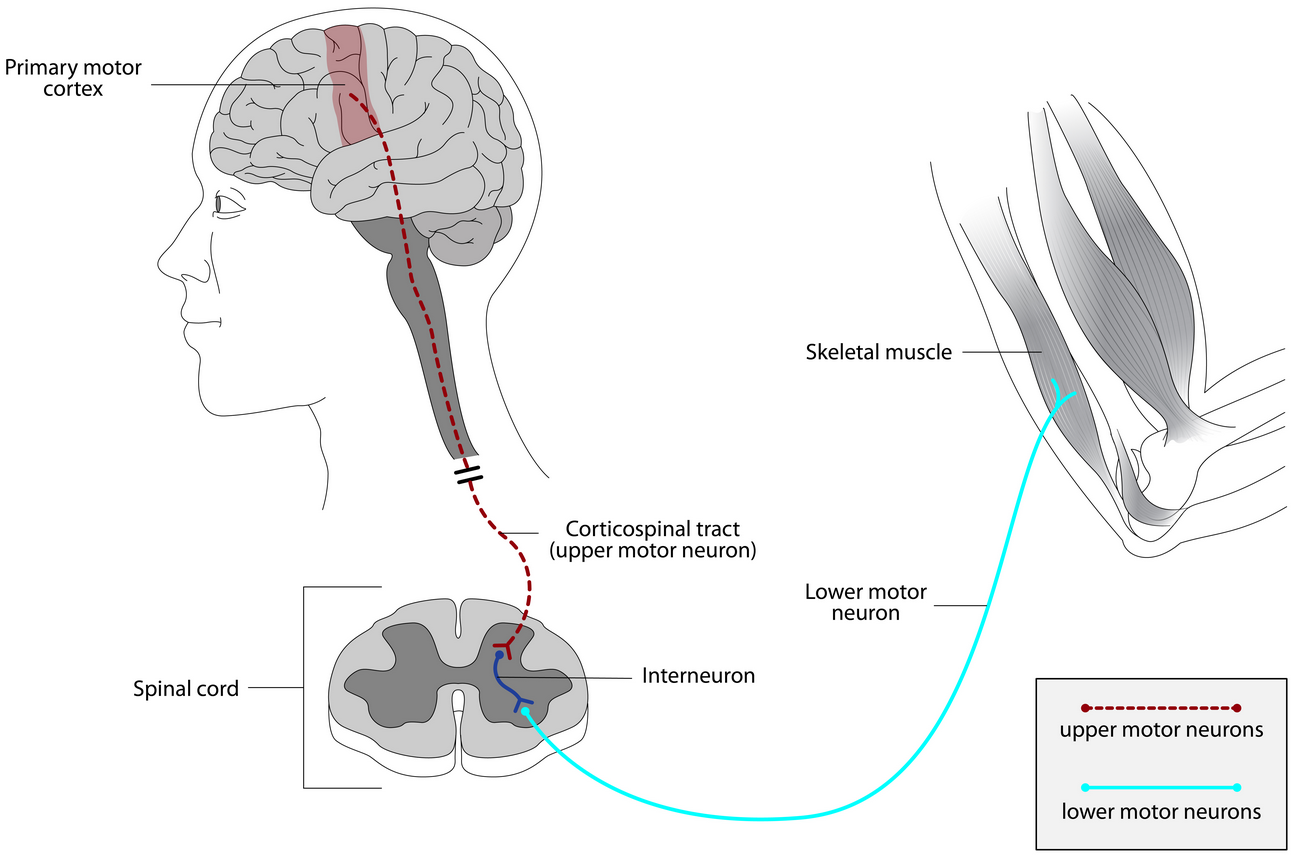
\includegraphics[width=1\linewidth]{Cortex_Spinal.jpg}
    \caption{\scriptsize{\textit{\underline{Atteinte neuronale dans la SLA(P.Wicks, 2024)}}}}
    \label{fig:Cortex}
\end{wrapfigure}

Une maladie rare se définit par une \hyperref[def:prevalence]{prévalence} de 0{,}05,\% dans la population générale.
 Quatre-vingts pour cent de ces maladies sont d’origine génétique~\textsuperscript{\cite{centre_constitutif_sla_de_tours_protocole_2020}},
 et la SLA en fait partie : elle touche un individu sur 20,000 en Europe~\textsuperscript{\cite{orphanet_prevalence_2023}},
  et sa prévalence mondiale varie de 1{,}57 à 11{,}8 pour 100,000 selon les pays, de l’Iran aux États-Unis~\textsuperscript{\cite{c_wolfson_et_al_global_2023}}.
C’est une maladie neurodégénérative causée par une atteinte du motoneurone central au niveau du cortex cérébral \textbf{(figure \ref{fig:Cortex})},
 et par une dégénérescence progressive des fonctions musculaires. Cette pathologie est très handicapante, tant sur le plan physique que social.
  En raison de sa gravité et des conséquences dévastatrices pour les patients et leur entourage, elle constitue un domaine de recherche de premier plan pour les généticiens. 
  C’est pourquoi il est pertinent d’intégrer une approche transcriptomique afin d’augmenter le rendement diagnostique des formes génétiques de la maladie et de mieux en comprendre les mécanismes.
Notons que les gènes responsables de la SLA sont globalement bien documentés. À ce jour, une quarantaine de gènes ont été identifiés et associés à la maladie. Dans 90\%
 des cas, leur implication est directe dans les formes familiales. Dans les 10\% restants, correspondant aux formes sporadiques, l’implication est plus indirecte, 
 via des perturbations de processus cellulaires clés tels que l’homéostasie de l’ARN, le transport axonal ou l’autophagie.
Enfin, on observe une forte hétérogénéité génétique, perceptible à travers l’implication de gènes aux fonctions parfois très différentes.,
 mais qui convergent toujours vers une dégénérescence neuronale. Les plus fréquemment impliqués sont  SOD1, TARDBP, FUS et C9ORF72~\textsuperscript{\cite{centre_constitutif_sla_de_tours_protocole_2020}},
  majoritaires dans la maladie ils constituent le socle des recherches génétiques pour tenter la mise au point de thérapies ciblées.

\subsection{Modéliser le signal biologique en données exploitables}

Supposons maintenant que l’on cherche à établir un profil d’expression génique pour notre quarantaine de gènes. 
Il faut alors s’interroger sur le support de lecture, c’est-à-dire le nombre de fois qu’une région d’ADN a été lue (ou comptée) au cours du séquençage.
On s'attend logiquement à avoir une densité de distribution de ces lectures, qui peut être intuitivement interprétée comme un reflet du niveau d’expression de chaque gène étudié.
En pratique, toutefois, un certain nombre de variables \textemdash ~ d’origine biologique ou expérimentale \textemdash ~ influencent cette expression théorique, introduisant une dispersion dans les données brutes.
A travers le schéma ci-dessous je présente un nombre non exhaustif de biais qui peuvent faussées l'expression génétique : 

\begin{figure}[ht]
    \centering
    \resizebox{0.8\textwidth}{!}{ 
    \begin{tikzpicture}[node distance=1.5cm and 1cm]

    \node (start) [startstop] {Prélèvement des échantillons : répétatibilité biologique ?};
    \node (step1) [process, below of=start, text width=6cm, align=center] {Extraction de l'ARN total};
    \node (step2) [process, below of=step1, text width=6cm, align=center] {Enrichissement de l'ARNm};
    \node (step3) [process, below of=step2, text width=6cm, align=center] {Fragmentation de l'ARN};
    \node (step4) [process, below of=step3, text width=6cm, align=center] {Synthèse de l'ADNc};
    \node (step5) [process, below of=step4, text width=6cm, align=center] {Préparation de la librairie};
    \node (step6) [process, below of=step5, text width=6cm, align=center] {Quantification de la librairie};
    \node (step7) [process, below of=step6, text width=6cm, align=center] {Séquençage};

    \node (note1) [techbias, right=3cm of step1, text width=6cm, align=center] {Pureté et Concentration extraite};
    \node (note2) [techbias, right=3cm of step2, text width=6cm, align=center] {Perte d'ARNm non poly-A};
    \node (note3) [techbias, right=3cm of step3, text width=6cm, align=center] {Fragmentation imparfaite};
    \node (note4) [techbias, right=3cm of step4, text width=6cm, align=center] {Efficacité reverse transcription};
    \node (note5) [techbias, right=3cm of step5, text width=6cm, align=center] {Thermocycleur, répétabilité};
    \node (note6) [techbias, right=3cm of step6, text width=6cm, align=center] {Variabilité de la quantification};
    \node (note7) [techbias, right=3cm of step7, text width=6cm, align=center] {Erreurs dues au séquençage};

    \draw [arrow] (start) -- (step1);
    \draw [arrow] (step1) -- (step2);
    \draw [arrow] (step2) -- (step3);
    \draw [arrow] (step3) -- (step4);
    \draw [arrow] (step4) -- (step5);
    \draw [arrow] (step5) -- (step6);
    \draw [arrow] (step6) -- (step7);

    \draw [arrow] (step1) -- (note1);
    \draw [arrow] (step2) -- (note2);
    \draw [arrow] (step3) -- (note3);
    \draw [arrow] (step4) -- (note4);
    \draw [arrow] (step5) -- (note5);
    \draw [arrow] (step6) -- (note6);
    \draw [arrow] (step7) -- (note7);

    %\node (note8) [biobias, right=0.5cm of step7, text width=2cm, align=center] {Illumina};
    %\node (note9) [biobias, right=0.2cm of step6, text width=2cm, align=center] {TapeStation};
    %\node (note10) [biobias, right=0.45cm of step5, text width=2cm, align=center] {Hamilton};
    %\node (note1) [biobias, right=0.5cm of step1, text width=2cm, align=center] {Nanodrop};

    % Ajout de la flèche verticale avec le texte "Processus"    
    \node[rectangle, rounded corners, draw=white, fill=gray!10, minimum width=10cm, minimum height=2cm, text width=2cm, align=center, anchor=north, rotate=90] at ([xshift=-5.4cm, yshift=-6cm]) {\textbf{Processus technique}};

    \end{tikzpicture}
    }
    \caption{\underline{\textit{ Schéma décisionnel pour normaliser les données RNASeq}}}
\end{figure}



\subsection{Etat de l'art}


\begin{figure}[ht]
\centering
\resizebox{1\textwidth}{!}{ 
\begin{tikzpicture}[node distance=1.5cm, every node/.style={font=\small}]

% ---------------------------------------------------
% Noeud de départ
\node (start) [smallbubble] {Quel objectif biologique ?};

% ---------------------------------------------------
% Questions initiales
\node (question1) [smallbubble, above left=1cm of start] {Comparaison globale ?};
\draw [arrow] (question1.south) |- (start.west);

\node (question2) [smallbubble, right=0.86cm of question1] {Analyse de gènes spécifique ?};
\draw [arrow] (question2.south) -- ++(0,0cm) -| (start.north);

\node (question3) [smallbubble, right=1cm of question2] {Quantification générale};
\draw [arrow] (question3.south) |- (start.east);

% ---------------------------------------------------
% Noeud de décision pour comparaison
\node (compare) [decision, below left=1.5cm of start] {Comparaison entre échantillons};
\draw [arrow] (start.south) |- (compare.east) node[midway, above, yshift=-1pt,xshift=-1.7cm] {\scriptsize{Soneson et al. 2016}};;

% ---------------------------------------------------
% Noeud de décision pour étude ciblée
\node (gene) [decision, below right=1.5cm of start] {Etude ciblée : un/des gènes};
\draw [arrow] (start.south) |- (gene.west) node[midway, above, yshift=-1pt,xshift=1.8cm] {\scriptsize{Zhao et al. 2021}};

% ---------------------------------------------------
% Méthodes de normalisation pour Comparaison
\node (TMM) [process, below=1.5cm of compare, xshift=-3cm] {TMM};
\node (RLE) [process, below=1.5cm of compare, xshift=2cm] {RLE};
\draw [arrow] (compare.south) -- ++(0,-1) -| (TMM.north);
\draw [arrow] (compare.south) -- ++(0,-1) -| (RLE.north);

% ---------------------------------------------------
% Références pour les méthodes de normalisation
\draw [arrow] (compare.south) -- ++(0,-1) -| (TMM.north) node[midway, right, yshift=6pt,xshift=-0.8cm] {\scriptsize{Robinson et al. 2010}};
\draw [arrow] (compare.south) -- ++(0,-1) -| (RLE.north) node[midway, right, yshift=6pt, xshift=-1.2cm] {\scriptsize{Anders et Huber 2010}};

% ---------------------------------------------------
% Formules sous les méthodes de normalisation
\node (TMMformula) [formula, below=2cm of TMM] {$TMM_{g,e} = \exp \left( \frac{\sum_{g} w_{g,e} M_{g,e}}{\sum_{g} w_{g,e}} \right)$};
\node (RLEformula) [formula, below=0.5cm of RLE] {$RLE_{ge} = \log_2\left(\frac{r_{ge}}{\text{Med}_g}\right)$};
\draw [arrow] (TMM.south) -- (TMMformula.north);
\draw [arrow] (RLE.south) -- (RLEformula.north);

% ---------------------------------------------------
% Méthodes de normalisation pour Quantification
\node (CPM) [process, below=1.5cm of gene,xshift=2cm] {CPM};
\node (FPKM_RPKM) [process, below left=1cm of CPM,xshift=-0.4cm] {FPKM \& RPKM};
\node (TPM) [process, below right=2cm and 0cm of CPM,minimum width=2cm] {TPM};

% ---------------------------------------------------
% Références pour les méthodes de quantification
\draw [arrow] (gene.south) -- ++(0,-1) -| (CPM.north) node[midway, right, yshift=6pt,xshift=-2cm] {\scriptsize{Anders et Huber 2010}};
\draw [arrow] (gene.south) -- ++(0,-1) -| (FPKM_RPKM.north) 
    node[midway, left, yshift=0.1cm, xshift=-0.3cm, rotate=90] {\scriptsize Mortazavi  2008}
    node[midway, right, yshift=-2.1cm, xshift=0.3cm, rotate=90] {\scriptsize{Derrien  2012}};

\draw [arrow] (gene.south) -- ++(0,-1) -| (TPM.north) node[midway, right, yshift=6pt,xshift=0.3cm,rotate=270] {\scriptsize{Parker et al. 2016}};

% ---------------------------------------------------
% Formules pour Quantification
\node (CPMformula) [formula, below=0.5cm of CPM] {$\displaystyle CPM_{g,e} = \frac{R_g}{\frac{\sum{r_e}}{\lambda}}$};
\node (FPKM_RPKMformula) [formula, below=1cm of FPKM_RPKM] {$\displaystyle FPKM_{g,e} = \lambda \times \frac{F_g}{L_g \times \sum_{e}F_e} $};
\node (TPMformula) [formula, below=1.5cm of TPM,xshift=0cm] {$TPM_{g,e} = \lambda \times \frac{{RPK}_{g,e}}{\sum_{e} \left(\frac{R_e}{L_e}\right)}$};

% Relier les flèches aux formules
\draw [arrow] (CPM.south) -- (CPMformula.north);
\draw [arrow] (FPKM_RPKM.south) -- (FPKM_RPKMformula.north);
\draw [arrow] (TPM.south) -- (TPMformula.north);

% ---------------------------------------------------
% Loi binomiale négative
\node (negBinom) [process, below=1.5cm of {$(RLEformula)!1!(TMMformula)$}] {Loi binomiale négative};
\draw [arrow] (negBinom.south) -- ++(0,-1);
% Relier les flèches des formules à la loi binomiale négative
\draw [arrow] (RLEformula.south) -- (negBinom.north) node[midway, above, yshift=-5pt, xshift=1.5cm] {\scriptsize{Duncan et al. 2009}}; 


% ---------------------------------------------------
% Formule de la loi binomiale négative
\node (LBNformula) [formula, below=1cm of negBinom] {$P(C_{g,e} = k) = \binom{r+k-1}{k} p^r (1-p)^k$};

% Relier la LBN à sa formule
\draw [arrow] (negBinom.south) -- (LBNformula.north); 

\end{tikzpicture}
}
\caption{\underline{\textit{ Schéma décisionnel pour normaliser les données RNASeq}}}
\end{figure}

 doivent elles être intégrées à l'analyse finale ? Cette question vas être pertinente dans une étude quantitative comme ici, puisqu'il s'agit, en autre, de caractériser une eventuelle haplo-insuffisance ou surexpression. 
 Nous allons comparer les différentes stratégies.Le périmètre de ce travail préliminaire était de faire un état des lieux des méthodes conventionnelles de normalisation,
pour \textit{in fine} détecter une éventuelle expression génétique différentielle à partir des données issues du séquençage RNA-Seq.
En effet, la transcription, étant fondatrice de la diversité protéomique, est par nature source de nombreuses anomalies génétiques. À l’issue de ce mécanisme,
un gène peut exprimer plusieurs isoformes dont l’impact peut être pathologique. Identifier de telles anomalies implique la création d’un protocole de séquençage spécifique et
d’un pipeline d’analyse RNA-Seq. L’objectif, à terme, est de déployer ce \textit{workflow} en intégrant une dimension transcriptomique pour le diagnostique de la SLA.\\
Durant mon premier semestre, j’ai eu l’occasion d’effectuer un travail de recherche bibliographique pour étayer ma compréhension des différentes approches permettant de mettre en œuvre cette étape.
La synthèse de ce travail préliminaire peut s’apprécier à travers la figure de synthèse ci-dessous :



Après avoir explorer les différentes méthodes de normalisation, en mettant particulièrement l'accent sur TMM, RLE et LBN, qui apportent une valeur ajoutée dans le contexte du RNA-Seq ciblé. Cette analyse repose sur plusieurs critères de performance clés en génétique, tels que les comparaisons inter-individuelles et la robustesse face aux valeurs extrêmes.
 L'objectif final etait d'évaluer l'approche la plus adaptée  d'un panel de gènes ciblés .

\subsection{Performance à faible profondeur et robustesse aux valeurs extrêmes} \vspace{3mm} Un des principaux critères d’évaluation est la robustesse aux valeurs extrêmes. Lorsqu’on cherche à établir un profil d'expression pour une maladie rare, comme la SLA, il est essentiel de déterminer si les valeurs de comptage aux extrémités de la distribution doivent être intégrées à l'analyse finale. Cette question peut être pertinente dans une étude quantitative visant à caractériser une éventuelle haplo-insuffisance ou surexpression. Nous allons comparer les différentes stratégies.\\

Les méthodes dites \textit{"Total Count"}, comme CPM, bien qu’utilisées pour leur simplicité, sont particulièrement sensibles aux valeurs extrêmes\textsuperscript{\cite{dillies_comprehensive_2013}}. Elles considèrent peu d'informations et ne permettent pas une évaluation efficace de la dispersion des données. Dans un contexte où l'expression génétique varie, elles se révèlent inadéquates. De même, FPKM et TPM présentent des limitations similaires. Ces méthodes sont souvent critiquées pour leur manque de reproductibilité et leur rigueur scientifique. Par exemple, \citeauthor{robinson_scaling_2010} (2010) ont montré que la division par la longueur du gène amplifie l’effet des valeurs aberrantes, surtout pour les gènes courts ou faiblement exprimés\textsuperscript{\cite{anders_differential_2010}}. Les travaux de \citeauthor{zhao_tpm_2021} (2021) confirment également cette limite. Quant à la méthode "Upper Quartile", cela est plus nuancé, car elle élimine les données du quartile inférieur\textsuperscript{\cite{dillies_comprehensive_2013}}, donc partiellement les valeurs extrêmes, mais elle reste peu adaptée à notre contexte où certains gènes peuvent être faiblement ou fortement exprimés par rapport à ce qui est attendu biologiquement.\\

A l'inverse, TMM, qui prend en compte la composition de l’ARN au moment de la normalisation, offre une meilleure résistance aux biais causés par les valeurs extrêmes\textsuperscript{\cite{robinson_scaling_2010}}. C'est aussi le cas pour RLE, grâce à l’utilisation de la médiane comme paramètre de position, qui donne une tendance centrale. Enfin, LBN repose sur l’hypothèse que les gènes ne sont pas différentiellement exprimés entre les conditions, ce qui renforce sa pertinence pour analyser les extrémités de la distribution. Ces trois approches partagent une philosophie commune : estimer le facteur de normalisation à partir d’un ensemble de gènes supposés stables.

\subsection{Compromis entre facilité d'interprétation et la pertinence biologique}

Après avoir fait un panorama des différentes stratégies mathématiques pour traiter les comptages bruts, il est évident que la diversité des méthodes peut paraître déroutante. Finalement, ce qui va être essentiel pour le biologiste, c'est de lui proposer une approche qui repose sur un compromis entre facilité d'interprétation et pertinence médicale. Le biologiste doit être en mesure de comprendre les corrections pour les relier aux décisions diagnostiques. Les méthodes conceptuellement simples comme CPM et UQ sont éliminées des options disponibles pour le périmètre de notre étude, car nous avons montré que, avec des échantillons présentant des variations biologiques importantes, la normalisation conduira à des conclusions erronées. Nous avons vu que les métriques comme TPM et FPKM sont des approches moins avancées que TMM, RLE et LBN, qui sont également plus simples à comprendre et à implémenter que les autres, mais elles manquent de correction statistique pour les comparaisons inter-échantillons.\\

En conclusion, la piste à creuser dans le périmètre de notre étude pencherait vers TMM ou RLE, et venir modéliser avec la LBN la surdispersion. Dans la littérature, il est régulièrement fait référence que la solution adéquate réside dans l'application d'une double correction\textsuperscript{\cite{robinson_scaling_2010}}. Comme nous l'avons souligné dans la méthodologie de la LBN, une fois que les biais techniques sont absorbés (par la correction RLE ou TMM), la méthode LBN peut être appliquée pour l'analyse de l'expression différentielle. Cette stratégie répondra à la fois à la problématique de la surdispersion et permettra d'obtenir une estimation précise de la variabilité inter-individuelle. Enfin, il est intéressant de mentionner que la taille de l'échantillon statistique (nombre de librairies) est directement corrélée à la puissance de la correction LBN. Comme souvent en statistique : plus les données seront consistantes plus la correction le sera également. Une piste de travail pour s'adapter aux contraintes de temps et de coût au laboratoire et pouvoir appliquer de manière crédible ces corrections serait donc de compiler (TMM ou RLE avec LBN) les données des diagnostics des librairies successives, semaine après semaine, pour augmenter la taille des données.
 Bien évidemment, cela doit se faire sous contrôle d'analyses statistiques pour valider une telle approche. 
C'est une option à envisager pour fournir un modèle probabiliste puissant pour l'analyse d'expression malgrès les contraintes organisationnelles (8 échantillons par expérience).


 doit être apprécié en considérant que chaque méthode a ses avantages et inconvénients, et le choix sera fait sur un certain nombre de critères,
  en tenant compte des spécificités des données et de l'objectif(s) biologique(s). Ce sujet sur la normalisation des données RNA-Seq dans le cadre du panel de gènes ciblés
   nous a permis de mettre en lumière la complexité de cette étape de normalisation des données RNA-Seq et la nécessité d'une collaboration étroite entre biologistes et bioinformaticiens 
   pour faire parler efficacement les résultats expérimentaux 


\subsection{Le problème}

Avant tout, rappelons que nous travaillons sur une maladie constitutionnelle. Par conséquent, il y a une très faible probabilité d'analyser des échantillons distincts pour un même patient à un intervalle de temps raisonnable, ce qui a peu de sens d'un point de vue de la génétique constitutionnelle, sauf dans des cas particuliers comme les études familiales. La notion de variabilité intra-individuelle est une qualité à étudier sur une matrice biologique identique. De manière générale, au laboratoire de génétique, il s'agit du sang, dans un milieu de transport adapté (tube STRECK pour l'ARN). Si ces conditions ne sont pas respectées, cela pourrait plutôt refléter une hétérogénéité biologique inhérente à une régulation de l'expression liée à la nature même du tissu, aux conditions de transport, à la variabilité de l'environnement analytique, avant même de songer à absorber les différents biais.
Il est donc fondamental d'avoir une planification expérimentale aussi standardisée que possible et d'un référencement complet et précis des biais biologiques connus et d'en évaluer leur impact.
Évaluer les biais biologiques et techniques est délicat. Comme nous l'avons vu plus haut, ils peuvent être confondus (préparation de la librairie, effets de lots, longueur des gènes, etc.).
La littérature aborde cet aspect sous des angles parfois différents, et les conclusions sont attribuées à des facteurs techniques et/ou biologiques, car il est difficile de faire la distinction. 
 Chaque expérience étant unique, chaque prélèvement l'est aussi, notamment par ses délais et ses modalités d'acheminement. Pour capturer au mieux ces sources de variabilité, et à travers les différentes études comparatives, 
 j'ai constaté que les méthodes les méthodes conventionnelles présentées en \textbf{figure 1} ne sont pas ou peu adapté au RNASeq ciblé pour faire de DGE. Ceci s'explique par leurs modalités de calcul, qui intègrent la dispersion et la comparaison inter-échantillons à l'échelle du transcriptome ~\textsuperscript{\cite{dillies_comprehensive_2013}}. TMM, en utilisant une moyenne tronquée des ratios de lectures pour calculer les facteurs de normalisation,
  va corriger efficacement les biais liés à la taille de la librairie (profondeur de séquençage notamment) et à la composition de l'ARN (régions riches en GC)\textsuperscript{\cite{abrams_protocol_2019}}.
 
    Présentation du jeu de données : 72 échantillons de transcriptomique ciblée (56 gènes SLA).
    Organisation en runs de séquençage (n = 8 par run).
    Limites méthodologique,  absence de gènes de référence stables, peu de données pour une normalisation robuste.
    Constats initiaux : forte variabilité de profondeur de lecture inter-run, faible reproductibilité.
